%!TEX root = ../Main.tex
This section will mark the conclusion of the preliminary work done in \cref{theorysec,hamilsec,greensec}. All the functions producing on-site Hamiltonians, hopping matrices, full Hamiltonians, band structures as well as self energy and Green's functions by recursion, will be used to get the transmission through the material.\\
 First of all a sentence as to what transmission is: Transmission is the probability of an electron being transported trough a specific region for a specific range of energies and thus how the region affects the overall current flow of electrons through the system as a whole. Below is an equation stating it formally
 \begin{align}\label{transformal}
    P(t)_{mn} = \left|\mel{m}{e^{i\mathbf{H}t/\hbar}}{n}\right|^2
\end{align}
where \(m,n\) is the density of states in each side of the region of interest (states going in/out) and \(e^{i\mathbf{H}t/\hbar}\) is the solution to the Green's function.\\
To give an overview and explain the different concepts of transmission this section will rely heavily on \cref{systemillu} where all the different parts of the system have been translated from the actual material into mathematical
 formalism in the shape of matrices. 
\begin{figure}
    \centering 
    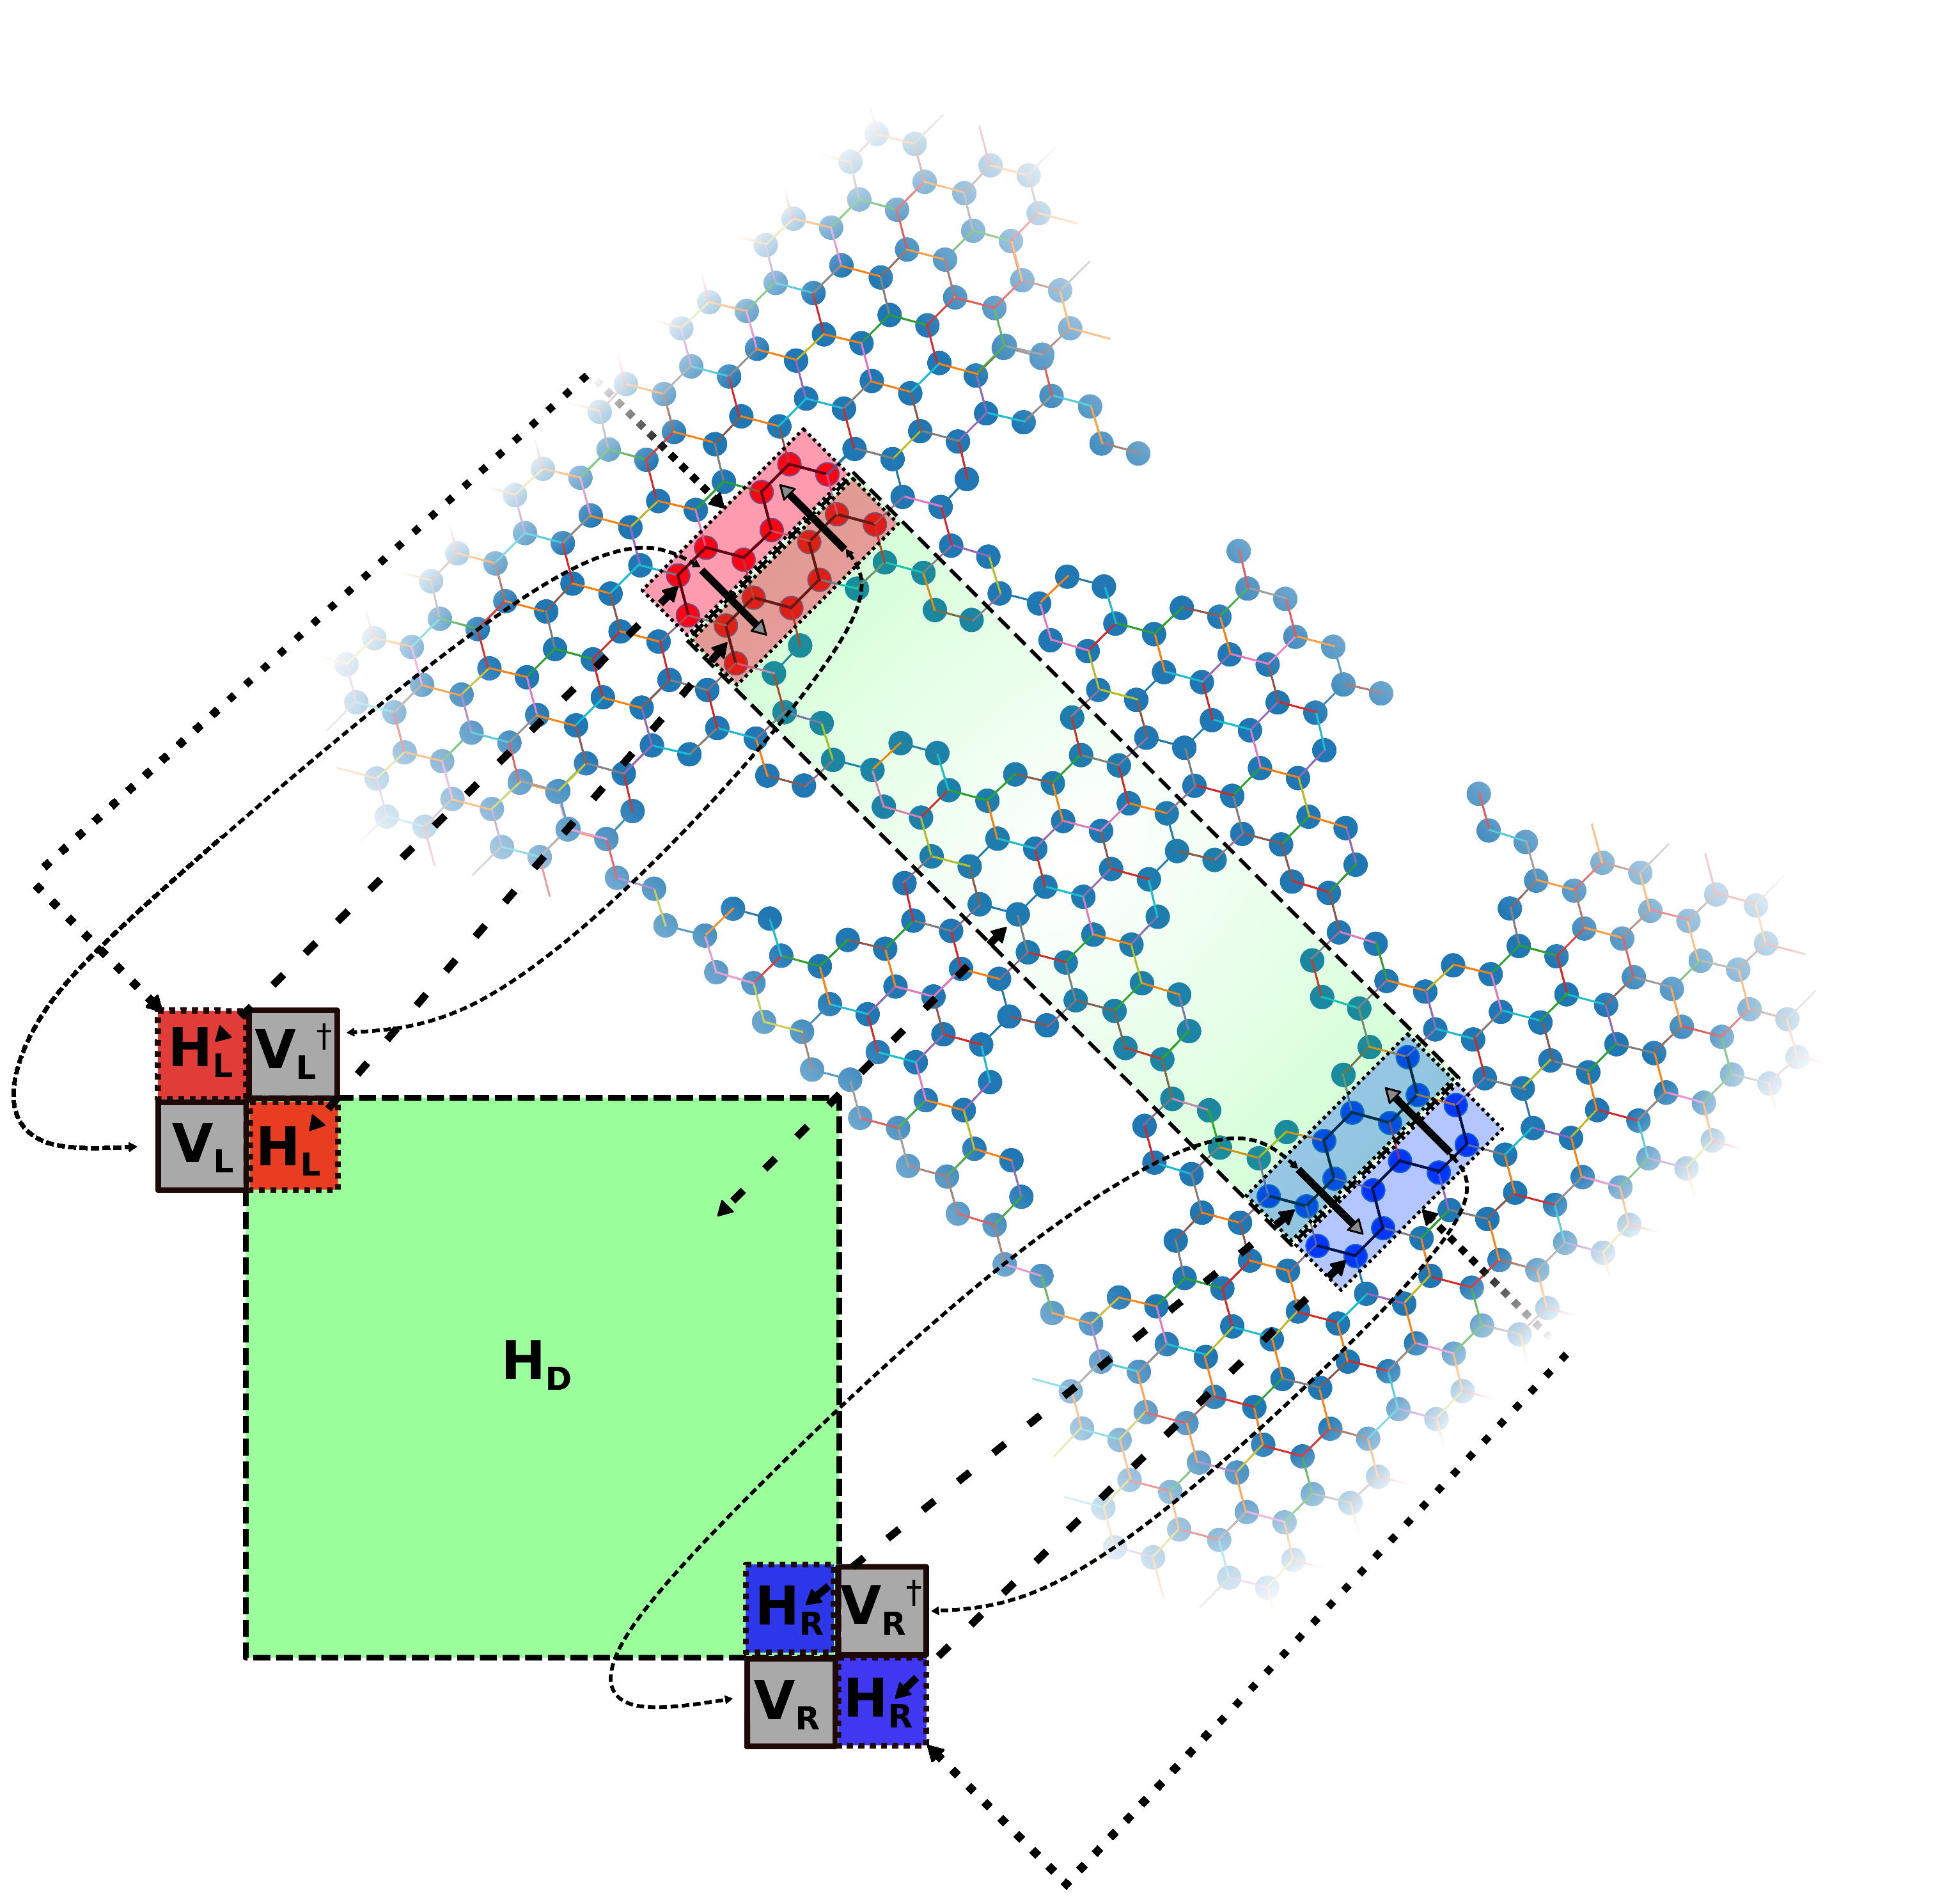
\includegraphics[width=0.9\textwidth]{Figures/illu.eps}
    \caption{Illustration showing how the different parts of the system are translated into matrix blocks in NPG. The green box is the unit cell of the device with the Hamiltonian \(\textbf{H}_D\). It includes one red and blue box which themselves are unit cells of the left and right contacts and have the Hamiltonians \(\textbf{H}_L,\ \textbf{H}_R\). The two other unit cells lying outside the device region represents what could be an infinite contact region reducible by recursion. Finally the two fat black arrows (not dotted) on each side of the device represents the hopping between the device- and contact region. Note that the direction of hopping corresponds to a specific hopping matrix. F.ex. left-to-right is the ordinary hopping matrix (\(\mathbf{V}\)) while right-to-left is its conjugate (\(\mathbf{V}^{\dagger}\)) (for both left and right side of the device).}
    \label{systemillu}
\end{figure}
The first and central piece is the so-called "Device Region" with the on-site Hamiltonian \(\mathbf{H}_D\) (Green area in \cref{systemillu}). The device region contains at least one central unit cell as well as a "left" and "right" unit cell (Red and blue area in \cref{systemillu}). The left and right unit cells represent the contact region of the device i.e. the two parts that connects to the rest of the system/molecule. They have on-site Hamiltonians \(\mathbf{H}_L,\mathbf{H}_R\) and they interact with rest of the system via hopping matrices \(\mathbf{V}_{L/R},\mathbf{V}^{\dagger}_{L/R}\). As \(\textbf{H}_D\) contains \(\textbf{H}_L,\ \textbf{H}_R\) they can be picked out of \(\textbf{H}_D, \)  without further calculation (See \cref{systemillu}) once the \(\mathbf{H}_D\) has been calculated. The cells next to the contact region can be reduced into a single Hamiltonian by recursion to have same dimension as \(\mathbf{H}_L,\mathbf{H}_R\). Note that \(\mathbf{H}_L,\mathbf{H}_R\) need not be the same dimensions.
Related to \(\mathbf{H}_L,\mathbf{H}_R\) is the left and right self energies \(\mathbf{\Sigma}_{L/R}\) and on-site Green's matrices \(\mathbf{g}_L\), \(\mathbf{g}_R\). These can be obtained using the theory and developed methods from \cref{greensec}. However the aim is to obtain the Green's matrix for the device region, \(\mathbf{G}_D\), as it is the one needed to fully describe the transmission in the region of interest. In other words, propagation of the states in the green area in \cref{systemillu}. To obtain it, one simply has to keep in mind that the effective coupling of the device region to the rest of the system is determined by the two contact regions (\(\mathbf{H}_L,\mathbf{H}_R\)) and thus the correction to the device Green's functions will be determined by the self energy of those contact regions. So the Green's matrix will be given by the same equation as \cref{Greenssolved} but with a self energy correction: 
\begin{align}\label{devicegreenseq}
    \mathbf{G}_D &= [\mathbf{1}(E+i\eta) - \mathbf{H}_D - \mathbf{\Sigma}_L(E) - \mathbf{\Sigma}_R(E)]^{-1} 
\end{align} 
Looking back at \cref{transformal} the Green's function needed has been obtained, but what about the states going in and out of the device region \(\bra{m}\ \text{and}\ \ket{n}\)? First thing needed to describe how the density of states pass through is by which rate they pass. To do this the rate operators \(\mathbf{\Gamma}_L,\mathbf{\Gamma}_R\) are introduced... They are given by
\begin{align}\label{rateeq}
\mathbf{\Gamma}_{L/R} = i(\mathbf{\Sigma}_{L/R} - \mathbf{\Sigma}^{\dagger}_{L/R})
\end{align}
Now the rate matrices have another important function as they can be used to rewrite the equation for the \textit{spectral function}:
\begin{align}\label{spectraleq}
    \mathbf{A}(E) &= -2\text{Im}[\mathbf{G}(E)] \\
    \downarrow \\
    \mathbf{A}(E) &= \mathbf{G}(E)\mathbf{\Gamma}(E)\mathbf{G}^{\dagger}(E)
\end{align}
To explain what the spectral function is, it is convenient to know that it too can be divided into two parts, a left and a right one. 
\begin{align}
    \mathbf{A}(E) &= \mathbf{A}(E)_L + \mathbf{A}(E)_R \\
    \mathbf{A}(E)_L &= \mathbf{G}(E)\mathbf{\Gamma}(E)_L\mathbf{G}^{\dagger}(E) \\ \mathbf{A}(E)_R &= \mathbf{G}(E)\mathbf{\Gamma}(E)_R\mathbf{G}^{\dagger}(E)
\end{align}
Taking the left spectral function as an example, it represents the density of states (note \cref{spectraleq}) of a wave coming from the left entering the device. Now one can also write the equation 
\begin{align}\label{lilletrans}
    \mathbf{A}_L(E)\mathbf{\Gamma}_R(E) = \mathbf{G}(E)\mathbf{\Gamma}(E)_L\mathbf{G}^{\dagger}(E)\mathbf{\Gamma}_R(E)
\end{align}
This corresponds to the density of states coming from the left, which then pass on through the right electrode by the rate \(\mathbf{\Gamma}_R(E)\) and because of time-reversal symmetry one can also get the density of states coming from the other direction. 
\begin{align}
    \mathbf{A}(E)_L\mathbf{\Gamma}(E)_R =  \mathbf{A}(E)_R\mathbf{\Gamma}(E)_L
\end{align}
This ultimately leads to transmission because transmission is in essence an expression of how much of the density of states passes trough the device and as explained \cref{lilletrans} is exactly the density of states, coming from the left (or right) and then passes through the right (left) by rate \(\mathbf{\Gamma}_{L/R}(E)\). So using the Green's function, left/right self energies as well as the left/right rate matrices, the transmission, as a function of energy, can be obtained via the following equation:
\begin{align}
    T(E) = \text{Tr}[\mathbf{\Gamma}_R\mathbf{G}_D\mathbf{\Gamma}_L\mathbf{G}_D^{\dagger}](E)
    \label{transeq}
\end{align}
Where Tr is the trace of the matrix product. 

\subsection{Transmission in 1D}
Again the developed routine in this section will be used on the simple system (\cref{pointplot}) as an example and in order to make sure that the obtained results are as expected. Thereafter it will be generalised to suit all kinds and sizes of system. First thing is to define the device in the same manner as \cref{systemillu} so that the device Hamiltonian \(\textbf{H}_D\) can be obtained through the already defined function \textit{Onsite}. The left and right Hamiltonian \(\textbf{H}_{L/R}\) are thus picked out as described earlier. An implementation has been made to the script to allow the user to see the left and right contact cells graphically as red and blue marked atom indices in the plot of the unit cell (See \cref{pointplot}).
This allows the user to get an overview of dimensions of \(\mathbf{H}_L,\mathbf{H}_R\) so they can be picked out of the device Hamiltonian correctly. From \(\mathbf{H}_L,\mathbf{H}_R\) the corresponding hopping matrices are defined using the \textit{Hop} function. Then the developed \textit{EnergyRecursion} function is used to obtain the device Green's matrix. This function is a more elaborate version of the earlier mentioned \textit{RecursionRoutine} and it takes \(\mathbf{H}_D,\mathbf{H}_L,\mathbf{H}_R,\mathbf{V}_L,\mathbf{V}_R\), a range of energies and \(\eta\) as inputs. It uses the old recursion routine to calculate the self energies for the left and right cells (\(\mathbf{\Sigma}_{L/R}\)) (see line xxx-xxx \cref{engrec}) and then uses those to calculate the device Green's function \(\textbf{G}_D\) as well as the left and right rate matrices \(\mathbf{\Gamma}_{L/R}\), using equations \cref{devicegreenseq}, \cref{} (see \cref{engrec} line xxx-xxx).\im{Listings/Functions.py}{156}{185}
\vspace{-1\baselineskip}
\captionof{listing}{Code showing how the device Green's functions as well as the left and right rate matrices are computed. First defining the different parts as described in the text above (line xx-xx), then looping over a range of energies (line xx-xx), using the old Recursion Routine and then inputting the self-energies in the equations from \cref{devicegreenseq} and \cref{rateeq} (line xx-xx). \label{engrec}}\vspace{\baselineskip}The output of the \textit{EnergyRecursion} function is the two rate matrices \(\mathbf{\Gamma}_{L/R}\) as well as the device Green's function \(\mathbf{G}_D\) and as per \cref{} the matrices needed for transmission have been obtained. As seen in \cref{transfunc} the function \textit{Transmission} simply carries out the matrix product and subsequent trace of the matrices resulting from \textit{EnergyRrecursion} and outputs a range of transmission probabilities which is then plotted against an energy range. Do mind that this is still just 1D in the sense that the transmission only moves in one direction. A plot of the transmission for the simple 1D system (the one in \cref{pointplot}) can be seen in \cref{Transsimple}.\im{Listings/Functions.py}{188}{195}
\vspace{-1\baselineskip}
\captionof{listing}{Code showing how the transmission probabilities are created. Taking in the rate matrices, device Green's function and a range of energies it takes the trace of the matrix product of for a range of energies as in \cref{transeq} (line xx-xx). \label{transfunc}}\vspace{\baselineskip}
\subsection{Development of transmission to 2D}\label{trans2d}
Lastly the transmission routine needs to be generalised so it can handle transport in two directions. The most convenient approach is to work with five real space unit cells as a starting point. One centre cell, a right and a left cell representing the contacts and then two additional cells on the left and right, representing the rest of the contact region. This would be the minimum amount of cells needed to generalise the transmission. One might have more center cells if the structure changes from one of those cells to the other. First these five unit cells will be defined using already developed tools. Then a big Hamiltonian, including all coordinates from the five cells representing real space are created, again using existing functions. One could call this big Hamiltonian \(\textbf{H}_{\text{Bigreal}}(x_0y_0z_0,x_0y_0z_0)\). It is a function of two sets of identical coordinates, namely the ones used to create the Hamiltonian itself. This has also been the case for all previous calculations, but the following steps will make it clear why it is explicitly stated for this Hamiltonian. The left/right on-site Hamiltonians and hopping matrices can thus be picked out of \(\textbf{H}_{\text{Bigreal}}(x_0y_0z_0,x_0y_0z_0)\) as before to get the Green's functions, self energies for transmission in real space, just as in the previous section. However, before the Green's function, self energies and transmission are calculated, the full left/right on-site Hamiltonian as well as their hopping matrices are defined as functions of a variable \(k\) which is added as a phase to the hopping matrices. As an example the following is the equation for the full right side Hamiltonian using the right on-side Hamiltonian with its hopping matrices: \(\textbf{H}_R(k) = \textbf{V}_Re^{ik}+\textbf{V}^{\dagger}_Re^{-ik}+\textbf{h}_R\). This added k-variable phase corresponds to transmission in the direction transverse to that in real space and it has \(2\pi\) periodic boundary conditions. This means that transport of electrons in the transverse direction in only dependent on a phase. However, one still needs the interaction between the centre on-site Hamiltonian (or device Hamiltonian) and the cells repeated in the transverse direction. Firstly the hopping between \(\textbf{H}_{\text{Bigreal}}(x_0y_0z_0,x_0y_0z_0)\) and a transversely shifted Hamiltonian is defined as \(\textbf{W} = \textbf{H}_{\text{Bigtrans}}(x_0y_0z_0,x_1y_1z_1)\) (Here using \textbf{W} as not to confuse it with \textbf{V} which is hopping between cells in real space). The  index of 1 in the second set of coordinates in \(\mathbf{W}\) is to mark that the original coordinates have been shifted in the transverse direction. With the hopping matrices \(\mathbf{W}\) for the transverse direction defined a Hamiltonian dependent on \(k\)-point values can be defined as:\begin{flalign}
    \textbf{H}(k) &= \textbf{h}+\textbf{W}e^{ik}+\textbf{W}^{\dagger}e^{-ik}\\ \nonumber
    &= \textbf{H}_{\text{Bigreal}}(x_0y_0z_0,x_0y_0z_0)+\textbf{H}_{\text{Bigtrans}}(x_0y_0z_0,x_1y_1z_1)e^{ik}+\textbf{H}_{\text{Bigtrans}}^{\dagger}(x_0y_0z_0,x_1y_1z_1)e^{-ik}
\end{flalign}
Now that a Hamiltonian, dependent of a variable \(k\) has been defined, it is now possible to get self energies, Green's functions that is \(k\)-dependent as well. This means that the transmission will also \(k\)-dependent. Thus transmission in 2D is essentially defined by a continuous variable in a range energies in real space and a continuous variable between \(-\pi,\pi\) in inverse space (transverse direction). This hereby concludes the all the initial effort to explain the formalism needed to get transmission in a two dimensional material such as NPG. Following is a walk through as to how this last step has been implemented through code programming.\\
To get the transmission in 2D the function \textit{PeriodicHamiltonian} is nested in a for loop, looping over transverse k-points (See \cref{trans2dcode} line xx-xx). The function \textit{PeriodicHamiltonian} basically translates the device Hamiltonian in the transverse direction (See \cref{appfigs},\cref{} for the code piece). Picked out from the resulting Hamiltonian is the left/right device Hamiltonian and left/right hopping matrix (See \cref{trans2dcode} line xx-xx. Still within the loop the \textit{EnergyRecursion} is used to get the device Greens function, and left/right rate matrices and lastly the transmission is done with the \textit{Transmission} function (\cref{trans2dcode} line xx) which is basically computing \cref{transmissioneq} as it stands. All these functions are used per k-point which effectively gives transmission in two dimensions.\im{Listings/NPGTransmission.py}{34}{72}
\vspace{-1\baselineskip}
\captionof{listing}{Code piece showing the transmission routine.}{\label{trans2dcode}}\vspace{\baselineskip}
Plots for transmission per k-point will be shown for NPG in \cref{CompTB}.
\subsection{Summary of Methodology}
\begin{figure}
    \centering
    \includegraphics[width=\textwidth]{Figures/Flowchart.eps}
    \caption{Flowchart depicting the routines run in python. SISL is used to import the geometry. Afterwards the coordinates are either used for band structure plots or for transmission plots. For the band structures, a Hamiltonian at each desired k-point is generated and diagonalised in order to get the eigen energies. These energies are then plotted. With transmission, a periodic Hamiltonian at various transverse k-points are generated and reduced to self energies in the transport direction (using the recursion algorithm). The self energies and the Green's functions retrieved here are then multiplied as to get the transmission.}
    \label{Flowchart}
\end{figure}
\subsection{Comparing Tight Binding with DFT and TBtrans for transmission and band structure calculations in NPG}\label{CompTB}
All the scripts necessary for calculation have been developed and they can now be used on a system of NPG.
The following results are based on this structure similar to that of \cref{atomrepfig}. Firstly the band structure obtained using the script described in \cref{FullHam} is shown together with  band plots obtained from DTF and TBtrans calculations. 
\begin{figure}[H]
	\centering
	\begin{subfigure}[t]{0.45\textwidth}
	\centering
		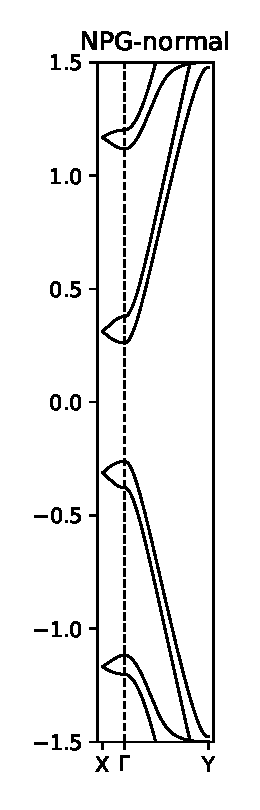
\includegraphics[width=0.5\textwidth]{Figures/NPG-normalBandstructures.eps}
		\caption{Figure showing the band structure for NPG with normal bridges obtained with the script described in \cref{FullHam}}
		\label{bsscript}
	\end{subfigure}
	~  %add desired spacing between images, e. g. ~, \quad, \qquad, \hfill etc.
	%(or a blank line to force the subfigure onto a new line)
	\begin{subfigure}[t]{0.45\textwidth}
	\centering
		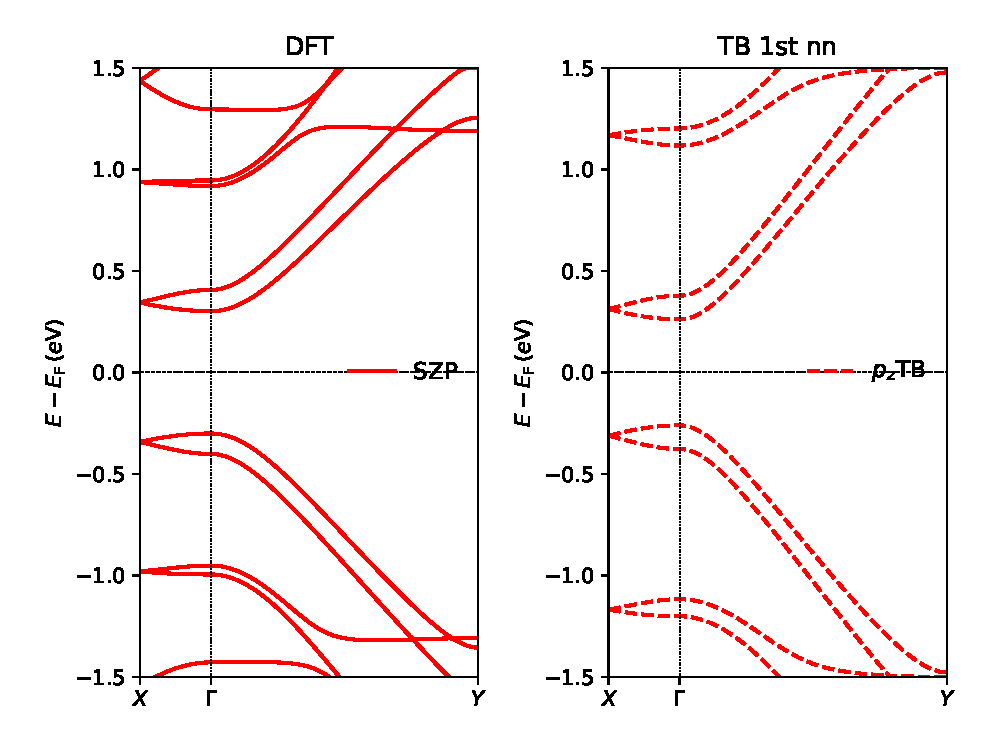
\includegraphics[width=\textwidth]{Figures/bands.eps}
		\caption{Figure showing the bands structures obtained from DFT and TBtrans calculations.}
		\label{bsdfttbt}
	\end{subfigure}
	\caption{Figure showing how the band plots compare for DFT, TBtrans and the developed script.}\label{bandcompare}
\end{figure}
The band plot obtained in \cref{bsscript} shows almost 1-to-1 correspondence with the plot obtained using TBtrans \cref{bsdfttbt} (right) and is also very similar to the plot obtained from DFT \cref{bsdfttbt} (left), proving that the script is capable of creating band structures for NPG-systems. Next is a comparison of the transmission in NPG for different k-points in reciprocal space. The plots are made for transmission through NPG in real space (x-direction) for each three different k-points in the reciprocal space (\(\dfrac{1}{y}\)-direction). The three k-points are \(0,\ \dfrac{\pi}{2},\ \pi\). Additionally an average over these k-points is plotted as well. In \cref{transmissionplots} transmission plots obtained with the script described in \cref{trans2d} is compared with transmission plot obtained through DTF, using the same k-points.
\begin{figure}[H]
	\centering
	\begin{subfigure}[b]{\textwidth}
        \centering
		\includegraphics[width=0.35\textwidth]{example-image-a}
		\qquad
		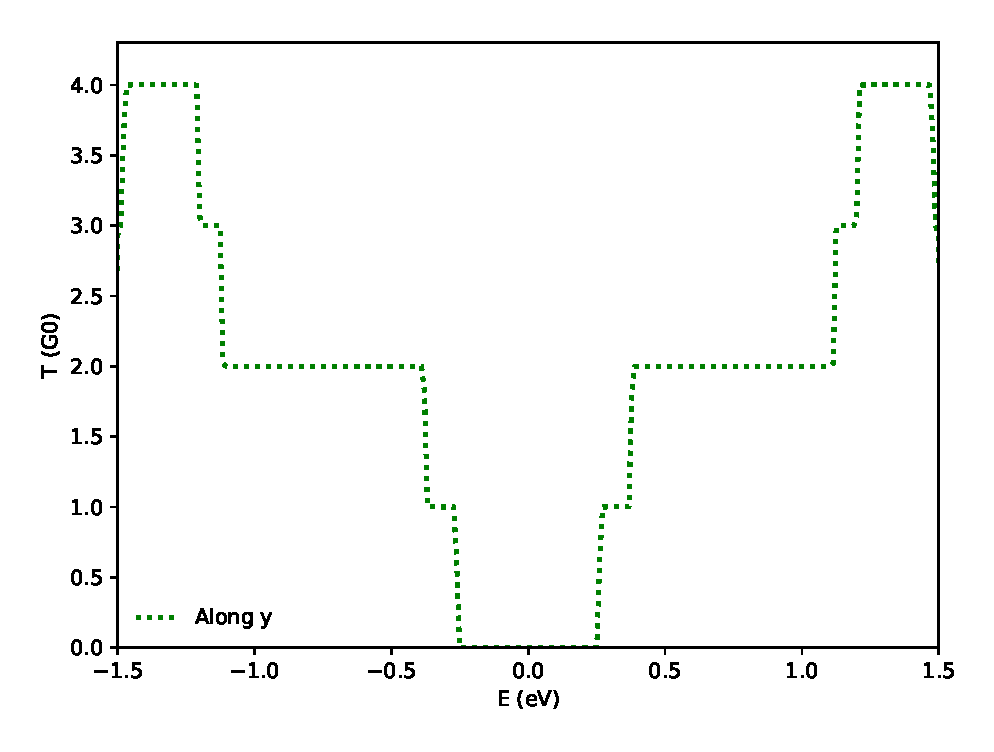
\includegraphics[width=0.35\textwidth]{Figures/txy_0.eps}
		\caption{Transverse k-point 0}
		\label{pizero}
	\end{subfigure}
	\vskip\baselineskip
	\begin{subfigure}[b]{\textwidth}
	    \centering
	    \includegraphics[width=0.35\textwidth]{example-image-c}
		\qquad
		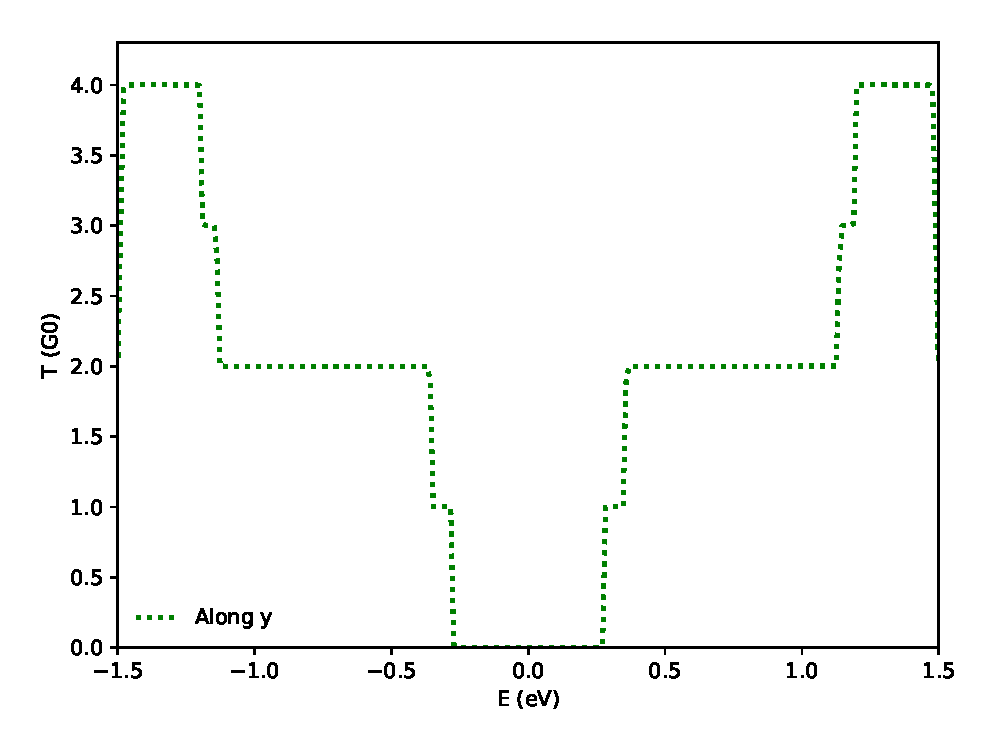
\includegraphics[width=0.35\textwidth]{Figures/txy_pi-half.eps}
		\caption{Transverse k-point \(\dfrac{\pi}{2}\)}
		\label{pihalf}
	\end{subfigure}
	\vskip\baselineskip
	\begin{subfigure}[b]{\textwidth}
	    \centering
	    \includegraphics[width=0.35\textwidth]{example-image-a}
		\qquad
		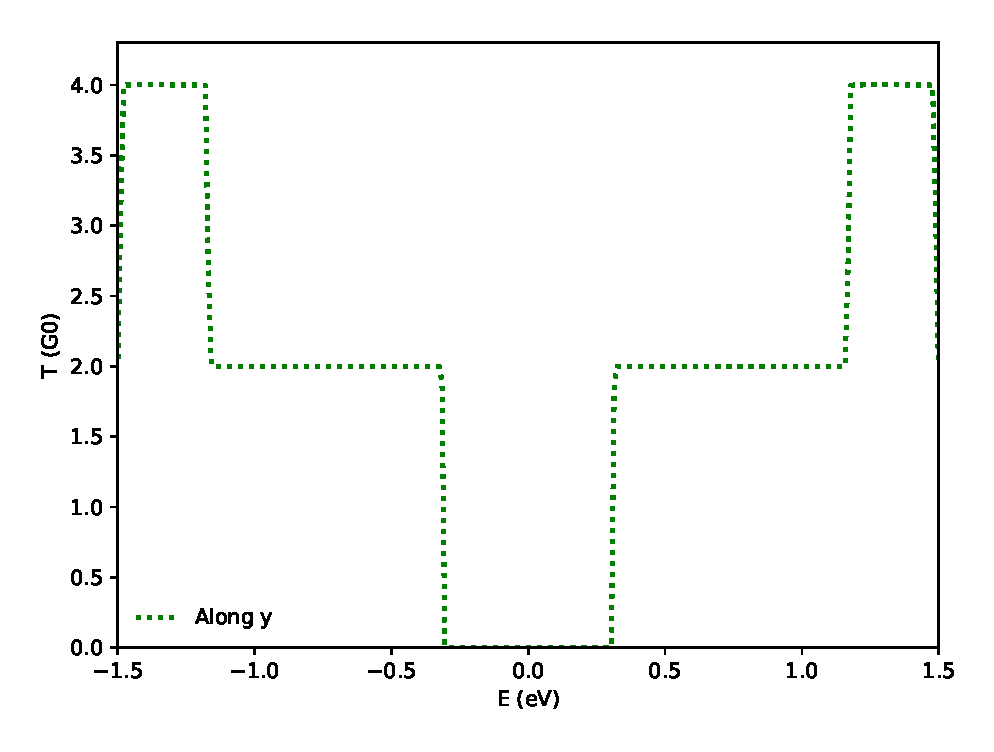
\includegraphics[width=0.35\textwidth]{Figures/txy_pi.eps}
		\caption{Transverse k-point \(\pi\)}
		\label{pi}
	\end{subfigure}
	\vskip\baselineskip
	\begin{subfigure}[b]{\textwidth}
	    \centering
	    \includegraphics[width=0.35\textwidth]{example-image-b}
		\qquad
		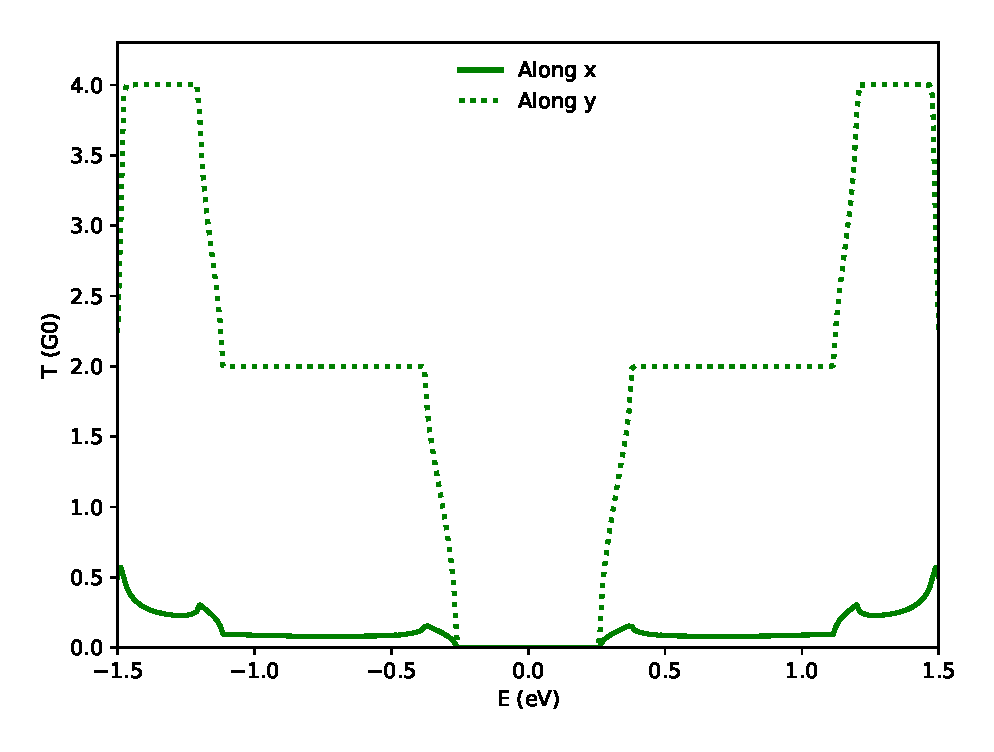
\includegraphics[width=0.35\textwidth]{Figures/txy_AVER.eps}
		\caption{Average over k-points \(0,\ \dfrac{\pi}{2},\ \pi \)}
		\label{piavg}
	\end{subfigure}
	\caption{Figure showing the comparison between plots of transmission through NPG obtained using the developed scripts (left/blue) and obtained using DFT (right/green).}\label{transmissionplots}
\end{figure}
As one can see in \cref{transmissionplots} The plots show very good correspondence with the DFT calculation. Again proving that the scripts developed on the basis of the Tight Binding approximation can produce valid results, when it comes to band structure and transmission through NPG.\\
This concludes the preliminary work. The tools for calculation of band structures, LDOS and transmission has been successfully developed, using \textit{python}-programming and the Tight Binding approximation. Following will be a range of tests on different NPG systems, using the developed tools. 
